% -*- latex -*-
%%%%%%%%%%%%%%%%%%%%%%%%%%%%%%%%%%%%%%%%%%%%%%%%%%%%%%%%%%%%%%%%
%%%%%%%%%%%%%%%%%%%%%%%%%%%%%%%%%%%%%%%%%%%%%%%%%%%%%%%%%%%%%%%%
%%%%
%%%% This text file is part of the source of 
%%%% `Introduction to High-Performance Scientific Computing'
%%%% by Victor Eijkhout, copyright 2012-7
%%%%
%%%% This book is distributed under a Creative Commons Attribution 3.0
%%%% Unported (CC BY 3.0) license and made possible by funding from
%%%% The Saylor Foundation \url{http://www.saylor.org}.
%%%%
%%%%
%%%%%%%%%%%%%%%%%%%%%%%%%%%%%%%%%%%%%%%%%%%%%%%%%%%%%%%%%%%%%%%%
%%%%%%%%%%%%%%%%%%%%%%%%%%%%%%%%%%%%%%%%%%%%%%%%%%%%%%%%%%%%%%%%

As a preliminary to OpenMP (section~\ref{sec:openmp}), we will briefly
go into `threads'.

To explain what a \emph{thread} is, we first need to get
technical about what a \indexterm{process} is.
A~unix process corresponds to the execution of a single program.
Thus, it has in memory:
\begin{itemize}
\item The program code, in the form of machine language instructions;
\item A \indexterm{heap}, containing for instance arrays that were
  created with \indextermtt{malloc};
\item A stack with quick-changing information, such as the
  \indexterm{program counter} that indicates what instruction is
  currently being executed, and data items with local scope, as well
  as intermediate results from computations.
\end{itemize}
This process can have multiple threads; these are similar
in that they see the same program code and heap, 
but they have their own stack. Thus, a thread is an independent
`strand' of execution through a process.

Processes can belong to different users, or be different
programs that a single user is running concurrently, so they
have their own data space.
On the other hand, threads are part of one process and
therefore share the process heap.
Threads can have some
private data, for instance by have their own data stack, but
their main characteristic is that they can collaborate on the same
data. 

\Level 2 {The fork-join mechanism}

Threads are dynamic, in the sense that they can be created during program 
execution. (This is different from the MPI model, where every processor
run one process, and they are all created and destroyed at the same time.)
When a program starts, there is one thread active: the \indextermsub{master}{thread}.
Other threads are created by \indextermbusdef{thread}{spawning}, and
the master thread can wait for their completion.
\begin{figure}[ht]
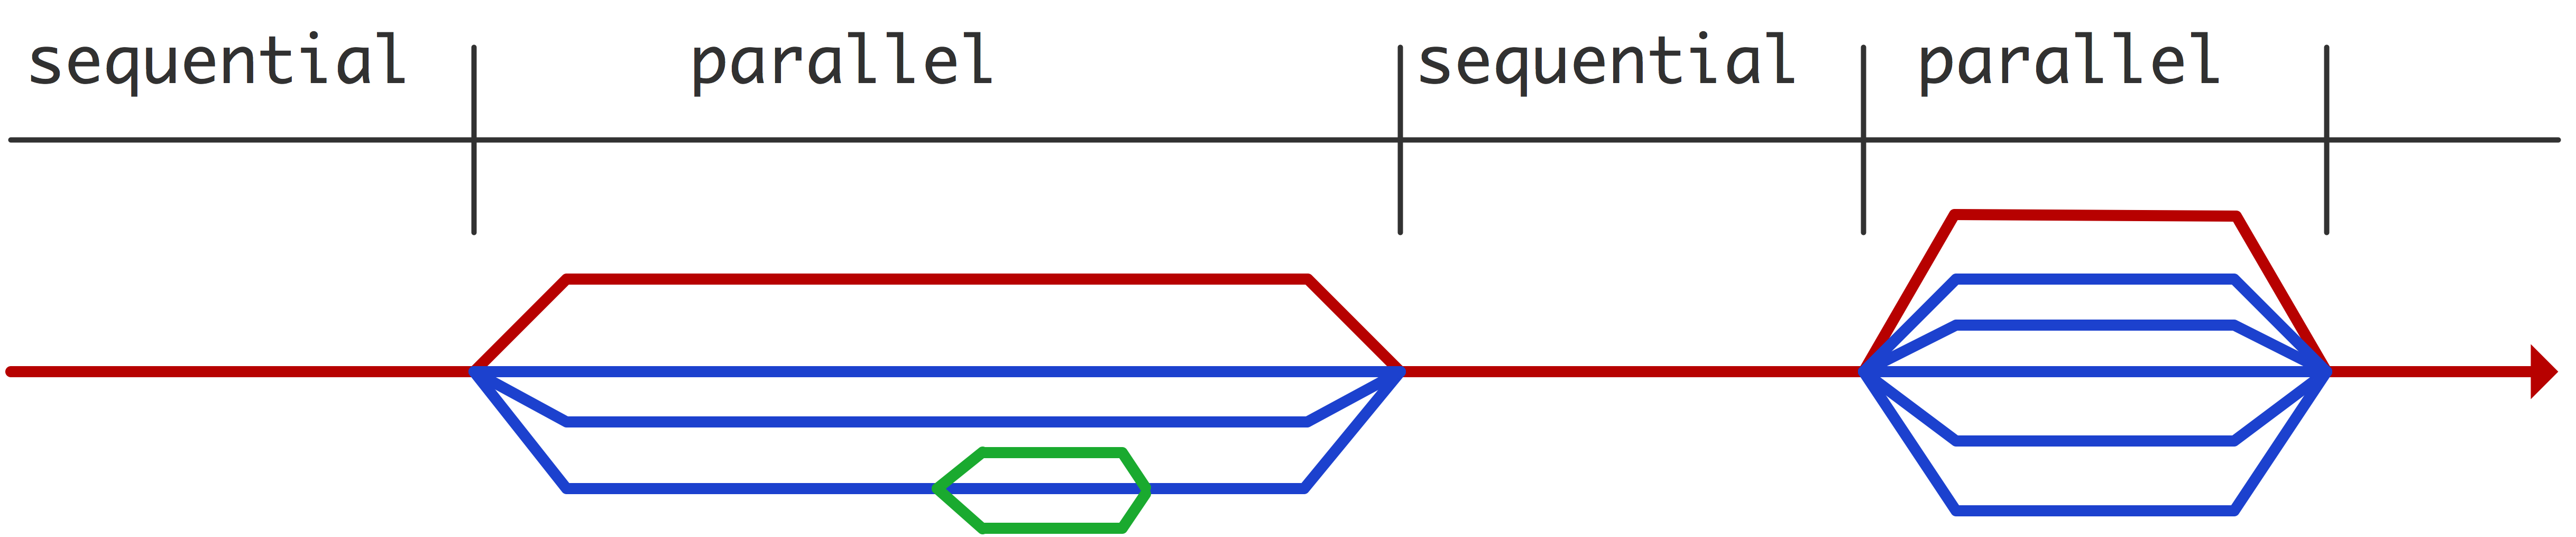
\includegraphics[scale=.08]{fork-join}
\caption{Thread creation and deletion during parallel execution}
\label{fig:forkjoin}
\end{figure}
This is known as the \indexterm{fork-join} model; it is illustrated
in figure~\ref{fig:forkjoin}. A~group of threads that is 
forked from the same thread and active simultaneously is known
as a \indextermbus{thread}{team}.

\Level 2 {Hardware support for threads}

Threads as they were described above are a software
construct. Threading was possible before parallel computers existed;
they were for instance used to handle independent activitives in an
\ac{OS}.
In the absence of parallel hardware, the \ac{OS} would handle
the threads through \indexterm{multitasking} or \indextermdef{time
  slicing}: each thread would regularly get to use the \ac{CPU} for a
fraction of a second. (Technically, the Linux kernel treads processes
and threads though the \indextermdef{task} concept; tasks are kept in
a list, and are regularly activated or de-activated.)

This can lead to higher processor utilization,
since the instructions of one thread can be processed
while another thread is waiting for data.
(On traditional CPUs,
switching between threads is somewhat expensive (an exception is the
\indexterm{hyperthreading} mechanism) but on \acp{GPU} it is not, and
in fact they \emph{need} many threads to attain high performance.)

On modern \indexterm{multicore} processors there is an obvious way of
supporting threads: having one thread per core gives a parallel
execution that uses your hardware efficiently. The shared memory allows the threads to all
see the same data. This can also lead to problems; see
section~\ref{sec:shared-lock}.

\Level 2 {Threads example}
\label{sec:thread-example}
\index{pthreads|(}

The following example
\begin{footnoteenv}
  {This is strictly Unix-centric and will
    not work on Windows.}
\end{footnoteenv}
is a clear illustration of the \indexterm{fork-join} model.
It uses the \emph{pthreads} library to spawn
a number of tasks that all update a global counter. Since threads
share the same memory space, they indeed see and update the same
memory location.
\begin{verbatim}
#include <stdlib.h>
#include <stdio.h>
#include "pthread.h"

int sum=0;

void adder() {
  sum = sum+1;
  return;
}

#define NTHREADS 50
int main() {
  int i;
  pthread_t threads[NTHREADS];
  printf("forking\n");
  for (i=0; i<NTHREADS; i++)
    if (pthread_create(threads+i,NULL,&adder,NULL)!=0) return i+1;
  printf("joining\n");
  for (i=0; i<NTHREADS; i++)
    if (pthread_join(threads[i],NULL)!=0) return NTHREADS+i+1;
  printf("Sum computed: %d\n",sum);

  return 0;
}
\end{verbatim}
The fact that this code gives the right result is a
coincidence: it
only happens because updating the variable is so much quicker than
creating the thread. (On a multicore processor the chance of errors
will greatly increase.) If we artificially increase the time for the
update, we will no longer get the right result:
\begin{verbatim}
void adder() {
  int t = sum; sleep(1); sum = t+1;
  return;
}
\end{verbatim}
Now all threads read out the value of \n{sum}, wait a while
(presumably calculating something) and then update.

This can be fixed by having a \indexterm{lock} on the code region that should be
`mutually exclusive':
\begin{verbatim}
pthread_mutex_t lock;

void adder() {
  int t;
  pthread_mutex_lock(&lock);
  t = sum; sleep(1); sum = t+1; 
  pthread_mutex_unlock(&lock);
  return;
}

int main() {
  ....
  pthread_mutex_init(&lock,NULL);

\end{verbatim}
The lock and unlock commands guarantee that no two threads can
interfere with each other's update.

For more information on pthreads, see for instance
\url{https://computing.llnl.gov/tutorials/pthreads}.

\index{pthreads|)}

\Level 2 {Contexts}
\label{sec:context}
\index{context|(textbf}

In the above example and its version with the \n{sleep} command
we glanced over the fact that there were two types of data involved.
First of all, the variable~\n{s} was created outside the thread spawning
part. Thus, this variable was \emph{shared}\index{thread!shared data}.

On the other hand, the variable~\n{t} was created once in each spawned thread.
We call this \emph{private}\index{thread!private data} data.

The totality of all data that a thread can access is called
its \emph{context}.  It contains private and shared data, as well as
temporary results of computations that the thread is working
on
\begin{footnoteenv}
  {It also contains the program counter and stack pointer. If
    you don't know what those are, don't worry.}
\end{footnoteenv}%
.

It is quite possible to create more threads than a processor has cores,
so a processor may need to switch between the execution of different threads.
This is known as a \indextermbusdef{context}{switch}.

Context switches are not for free on regular CPUs, so they only pay off
if the \indexterm{granularity} of the threaded work is high enough.
The exceptions to this story are:
\begin{itemize}
\item CPUs that have hardware support for multiple threads, for
  instance through \indexterm{hyperthreading}
  (section~\ref{sec:hyperthread}), or as in the
  \indextermbus{Intel}{Xeon Phi} (section~\ref{sec:copprocessor});
\item \acp{GPU}, which in fact rely on fast context switching (section~\ref{sec:gpu});
\item certain other `exotic' architectures such as the \indextermbus{Cray}{XMT}
  (section~\ref{sec:mta}).
\end{itemize}

\index{context|)}

\Level 2 {Data races, thread safety, and atomic operations}
\index{atomic operation|(}
\index{atomicity|see{atomic operation}}
\label{sec:shared-lock}

Shared memory makes life easy for the programmer, since every
processor has access to all of the data: no explicit data traffic
between the processor is needed. On the other hand, multiple
processes/processors can also write to the same variable, which is a
source of potential problems.

Suppose that two processes both try to increment an integer
variable~\texttt{I}:
\begin{tabbing}
  process 1: \texttt{I=I+2}\\
  process 2: \texttt{I=I+3}
\end{tabbing}
This is a legitimate activity if the variable is an accumulator for
values computed by independent processes.
The result of these two updates
depends on the sequence in which the processors read and
write the variable. Here are three scenarios:

\begin{tabular}{|rr|rr|rr|}
  \hline
  \multicolumn{2}{|c|}{scenario 1.}& \multicolumn{2}{|c|}{scenario 2.}&
  \multicolumn{2}{|c|}{scenario 3.}\\ \hline
  \multicolumn{6}{|c|}{$\n{I}=0$}\\ \hline
  read $\n{I}=0$&read $\n{I}=0$&
    read $\n{I}=0$&read $\n{I}=0$&
      read $\n{I}=0$& \\
  compute $\n{I}=2$&compute $\n{I}=3$& 
    compute $\n{I}=2$&compute $\n{I}=3$&
      compute $\n{I}=2$& \\
  write $\n{I}=2$& & &write $\n{I}=3$&write $\n{I}=2$& \\
  &write $\n{I}=3$&write $\n{I}=2$& & &read $\n{I}=2$\\
  &&&&&compute $\n{I}=5$\\
  &&&&&write $\n{I}=5$\\
  \hline
  \multicolumn{2}{|c|}{$\n{I}=3$}& \multicolumn{2}{|c|}{$\n{I}=2$}&
  \multicolumn{2}{|c|}{$\n{I}=5$}\\ \hline
\end{tabular}
Such a scenario, where the final result depends on which thread
executes first, is known as a \indexterm{race condition} or
\emph{data race}\index{data race|see{race condition}}.

A very practical example of such conflicting updates is the inner
product calculation:
\begin{verbatim}
for (i=0; i<1000; i++)
   sum = sum+a[i]*b[i];
\end{verbatim}
Here the products are truly independent, so we could choose to have
the loop iterations do them in parallel, for instance by their own
threads. However, all threads need to update the same variable~\n{sum}.

Code that behaves the same whether it's executed
sequentially or threaded is called \indextermbusdef{thread}{safe}.
As you can see from the above examples, a lack of thread safety is
typically due to the treatment of shared data. This implies that
the more your program uses local data, the higher the chance
that it is thread safe. Unfortunately, sometimes the threads need
to write to shared/global data, for instance when the program
does a \emph{reduction}\index{reduction!and thread safety}.

There are essentially two ways of solving this problem. 
One is that we declare such updates of a shared variable a
\indexterm{critical section} of code. This means that the instructions
in the critical section (in the inner product example `read \n{sum}
from memory, update it, write back to memory') can be executed by only
one thread at a time. In particular, they need to be executed
entirely by one thread before any other thread can start them so the
ambiguity problem above will not arise. Of course, the above code
fragment is so common that systems like OpenMP
(section~\ref{sec:openmp}) have a dedicated mechanism for it, by
declaring it a \emph{reduction}\index{reduction!under multi-threading}
operation.

Critical sections can for instance be implemented through the 
\indexterm{semaphore}
mechanism~\cite{Dijkstra:semaphores}. Surrounding each critical
section there will be two atomic operations controlling a semaphore, a
sign post.
The first process to encounter the semaphore will lower it, and start
executing the critical section. Other processes see the lowered
semaphore, and wait. When the first process finishes the critical
section, it executes the second instruction which raises the
semaphore, allowing one of the waiting processes to enter the critical
section.

The other way to resolve common access to shared data is to set a 
temporary \indextermdef{lock} on certain memory areas. This solution may
be preferable, if common execution of the critical section is likely,
for instance if it implements writing to a database or hash table. In
this case, one process entering a
critical section would prevent any other process from writing
to the data, even if they might be writing to different locations;
locking the specific data item being accessed is then a better
solution.

The problem with locks is that they typically exist on the operating
system level. This means that they are relatively slow. Since we hope that
iterations of the inner product loop above would be executed at the
speed of the floating point unit, or at least that of the memory bus,
this is unacceptable.

One implementation of
this is \indexterm{transactional memory}, where the hardware itself
supports atomic operations; the term derives from database
transactions, which have a similar integrity problem. In transactional
memory, a process will perform a normal memory update, unless the
processor detects a conflict with an update from another process. In
that case, the updates (`transactions') are aborted and retried with
one processor locking the memory and the other waiting for the
lock. This is an elegant solution; however, aborting the transaction
may carry a certain cost of \indextermsub{pipeline}{flushing}
(section~\ref{sec:pipelinecpu}) and
cache line invalidation (section~\ref{sec:coherence}).

\index{atomic operation|)}

\Level 2 {Memory models and sequential consistency}
\label{sec:seq-consist}

The above signaled phenomenon of a \indexterm{race condition}
means that the result of some programs can be non-deterministic,
depending on the sequence in which instructions are executed.
There is a further factor that comes into play, and which is
called the \indextermbus{memory}{model} that a processor and/or a
language uses~\cite{AdveBoehm:memorymodels}.
The memory model controls how the activity of one thread or core
is seen by other threads or cores.

As an example, consider
\begin{tabbing}
  initially: \texttt{A=B=0;}, then\\
  process 1: \texttt{A=1; x = B;}\\
  process 2: \texttt{B=1; y = A;}
\end{tabbing}
As above, we have three scenarios, which we describe by
giving a global sequence of statements:

\begin{tabular}{|l|l|l|}
  \hline
  scenario 1.& scenario 2.& scenario 3.\\ \hline
  $\n{A}\leftarrow \n{1}$&$\n{A}\leftarrow \n{1}$&$\n{B}\leftarrow \n{1}$\\
  $\n{x}\leftarrow \n{B}$&$\n{B}\leftarrow \n{1}$&$\n{y}\leftarrow \n{A}$\\
  $\n{B}\leftarrow \n{1}$&$\n{x}\leftarrow \n{B}$&$\n{A}\leftarrow \n{1}$\\
  $\n{y}\leftarrow \n{A}$&$\n{y}\leftarrow \n{A}$&$\n{x}\leftarrow \n{B}$\\
  \hline
  $x=0, y=1$& $x=1,y=1$& $x=1,y=0$\\
  \hline
\end{tabular}

(In the second scenario, statements 1,2 can be reversed, as can 3,4,
without change in outcome.)

The three different outcomes can be characterized as being computed by a global ordering
on the statements that respects the local orderings. This is known as \indexterm{sequential
  consistency}: the parallel outcome is consistent with a sequential execution that
interleaves the parallel computations, respecting their local statement orderings.

Maintaining sequential consistency is expensive: it means that any change to a variable
immediately needs to be visible on all other threads, or that any access to a variable
on a thread
needs to consult all other threads. We discussed this in section~\ref{sec:coherence}.

In a \indextermsub{relaxed}{memory model} it is possible to get a result that
is not sequentially consistent. Suppose, in the above example, the instructions
$\n{A}\leftarrow \n{1}$, $\n{B}\leftarrow \n{1}$ are executed first, but
these changes are not immediately visible to the other threads.
Then subsequent instructions
$\n{x}\leftarrow \n{B}$, $\n{y}\leftarrow \n{A}$  can receive the
result $x=0,y=0$, which was not possible under the sequentially consistent
model above.

Sequential consistency implies that
\begin{verbatim}
integer n
n = 0
!$omp parallel shared(n)
n = n + 1
!$omp end parallel
\end{verbatim}
should have the same effect as
\begin{verbatim}
n = 0
n = n+1 ! for processor 0
n = n+1 ! for processor 1
        ! et cetera
\end{verbatim}
With sequential consistency it is no longer necessary to declare
atomic operations or critical sections; however, this puts strong
demands on the implementation of the model, so it may lead to
inefficient code.

\begin{exercise}
  In section~\ref{sec:shared-lock} you saw an example that needed
  a critical section to get the right final result. Argue that
  having a critical section is not enough for sequential consistency.
  \begin{itemize}
  \item Write a piece of sequential code that, when executed in parallel,
    corresponds to the example in section~\ref{sec:shared-lock}.
  \item Show that, using a critical section, there are two execution
    orderings that give the correct result.
  \item Show that one of these orderings is not sequentially consistent.
  \end{itemize}
\end{exercise}

\Level 2 {Affinity}
\index{affinity|(}

Thread programming is very flexible, effectively creating parallelism
as needed. However, a large part of this book is about the importance
of data movement in scientific computations, and that aspect can not
be ignored in thread programming.

In the context of a multicore processor, any thread can be scheduled
to any core, and there is no immediate problem with this. However, if
you can about high performance, this flexibility can have unexpected
costs. There are various reasons why you want to certain threads to
run only on certain cores. Since the \ac{OS} is allowed to
\emph{migrate threads}\index{thread!migration}, may be you simply want
threads to stay in place.

\begin{itemize}
\item If a thread migrates to a different core, and that core has its
  own cache, you lose the contents of the original cache, and
  unnecessary memory transfers will occur.
\item If a thread migrates, there is nothing to prevent the OS from
  putting two threads on one core, and leaving another core completely
  unused. This obviously leads to less than perfect speedup, even if
  the number of threads equals the number of cores.
\end{itemize}

We call \emph{affinity} the mapping between
threads (\emph{thread affinity}\index{thread!affinity|see{affinity}})
or processes (\emph{process
  affinity}\index{process!affinity|see{affinity}}) and cores.
Affinity is usually expressed as a \emph{mask}\index{affinity!mask}: a
description of the locations where a thread is allowed to run.

As an example, consider a two-socket node, where each socket has four
cores.

With two threads and socket affinity we have the following affinity mask:\\
\begin{tabular}{|l|l|l|}
  \hline
  thread & socket 0 & socket 1\\
  \hline \hline
  0 & 0-1-2-3 & \\
  1 & & 4-5-6-7 \\
  \hline
\end{tabular}

With core affinity the mask depends on the affinity type. The typical
strategies are `close' and `spread'. With \indextermsub{close}{affinity}, the mask
could be:\\
\begin{tabular}{|l|l|l|}
  \hline
  thread & socket 0 & socket 1\\
  \hline \hline
  0 & 0 & \\
  1 & \hphantom{0-}1 & \\
  \hline
\end{tabular}

Having two threads on the same socket means that they probably share
an L2~cache, so this strategy is appropriate if they share data.

On the other hand, with \indextermsub{spread}{affinity} the threads
are placed further apart:\\
\begin{tabular}{|l|l|l|}
  \hline
  thread & socket 0 & socket 1\\
  \hline \hline
  0 & 0 & \\
  1 & & 4 \\
  \hline
\end{tabular}

This strategy is better for bandwidth-bound applications, since now
each thread has the bandwidth of a socket, rather than having to share
it in the `close' case.

If you assign all cores, the close and spread strategies lead to
different arrangements:\\
\begin{tabular}{|l|l|}
  \hline
  socket 0 & socket 1\\
  \hline \hline
  0-1-2-3 & \\
  & 4-5-6-7\\
  \hline
\end{tabular}

versus\\
\begin{tabular}{|l|l|}
  \hline
  socket 0 & socket 1\\
  \hline \hline
  0-2-4-6 & \\
  & 1-3-5-7 \\
  \hline
\end{tabular}

\heading{Affinity and data access patterns}

Affinity can also be considered as a strategy of binding execution to data.

Consider this code:
\begin{verbatim}
for (i=0; i<ndata; i++) // this loop will be done by threads
  x[i] = ....
for (i=0; i<ndata; i++) // as will this one
  ... = .... x[i] ...
\end{verbatim}
The first loop, by accessing elements of~$x$, bring memory into cache
or page table. The second loop accesses elements in the same order, so
having a fixed affinity is the right decision for performance.

In other cases a fixed mapping is not the right solution:
\begin{verbatim}
for (i=0; i<ndata; i++) // produces loop
  x[i] = ....
for (i=0; i<ndata; i+=2) // use even indices
  ... = ... x[i] ...
for (i=1; i<ndata; i+=2) // use odd indices
  ... = ... x[i] ...
\end{verbatim}
In this second example, either the program has to be transformed, or
the programmer has to maintain in effect a \indextermbus{task}{queue}.


\heading{First touch}

It is natural to think of affinity in terms of `put the
execution where the data is'. However, in practice the opposite view
sometimes makes sense.  For instance, figure~\ref{fig:ranger-numa}
showed how the shared memory of a cluster node can actually be
distributed. Thus, a thread can be attached to a socket, but data can
be allocated by the \ac{OS} on any of the sockets.  The mechanism that
is often used by the \ac{OS} is called the \indextermdef{first-touch}
policy:
\begin{itemize}
\item When the program allocates data, the \ac{OS} does not actually
  create it;
\item instead, the memory area for the data is created the first
  time a thread accesses it;
\item thus, the first thread to touch the area in effect causes the
  data to be allocated on the memory of its socket.
\end{itemize}

\begin{exercise}
  Explain the problem with the following code:
\begin{verbatim}
// serial initialization
for (i=0; i<N; i++)
  a[i] = 0.;
#pragma omp parallel for
for (i=0; i<N; i++)
  a[i] = b[i] + c[i];
\end{verbatim}
\end{exercise}

For an in-depth discussion of memory policies, see~\cite{Lameter:NUMAq}.

\index{affinity|)}

\Level 2 {Cilk Plus}

Other programming models based on threads exist. For instance,
Intel \indexterm{Cilk Plus} (\url{http://www.cilkplus.org/})
is a set of extensions of C/C++ with which a
programmer can create threads.

\hbox{%
  \kern.5\unitindent
  \begin{minipage}{2in}\tt
    \begin{tabbing}
      \textit{Sequential code:}\\  
      int \=fib(int n)\{ \\
      \>if (n<2) return 1;\\
      \>else \=\{\\
      \>\>int rst=0;\\
      \>\>rst += fib(n-1);\\
      \>\>rst += fib(n-2);\\
      \>\>return rst;\\
      \>\>\}\\
      \}\\
    \end{tabbing}
      \end{minipage}
  \kern.5\unitindent
  \begin{minipage}{2in}\tt
    \begin{tabbing}
      \textit{Cilk code:}\\  
      cilk int \=fib(int n)\{ \\
      \>if (n<2) return 1;\\
      \>else \=\{\\
      \>\>int rst=0;\\
      \>\>rst += cilk\_spawn fib(n-1);\\
      \>\>rst += cilk\_spawn fib(n-2);\\
      \>\>cilk\_sync;\\
      \>\>return rst;\\
      \>\>\}\\
      \}\\
    \end{tabbing}
      \end{minipage}
}

In this example, the variable \n{rst} is updated by two, potentially
independent threads. The semantics of this update, that is, the
precise definition of how conflicts such as simultaneous writes are
resolved, is defined by \indexterm{sequential consistency}; see
section~\ref{sec:seq-consist}.

\Level 2 {Hyperthreading versus multi-threading}
\label{sec:hyperthread}
\index{hyperthreading|(textbf}
\index{Symmetric Multi Threading|see{hyperthreading}}

In the above examples you saw that the threads that are spawned during one 
program run essentially execute the same code, and have access to the same data.
Thus, at a hardware level, a thread is uniquely determined by a small number of
local variables, such as its location in the code (the \indexterm{program counter})
and intermediate results of the current computation it is engaged in.

Hyperthreading is an Intel technology to let multiple threads use the
processor truly simulateneously, so that part of the processor would
be optimally used.
%% ; see figure~\ref{fig:hyperthread}.
%% \begin{figure}
%% 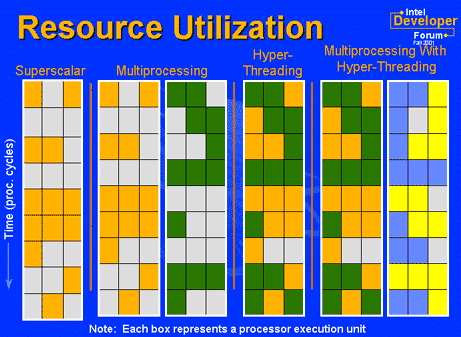
\includegraphics[scale=.6]{hyperthreading_image1}
%% \caption{Illustration of processor utilization under hyperthreading.}
%% \label{fig:hyperthread}
%% \end{figure}

If a processor switches between executing one thread and another, it saves this
local information of the one thread, and loads the information of the other.
The cost of doing this is modest compared to running a whole program, but 
can be expensive compared to the cost of a single instruction. Thus,
hyperthreading may not always give a performance improvement.

Certain architectures have support
for \indexterm{multi-threading}. This means that the hardware actually
has explicit storage for the local information of multiple threads,
and switching between the threads can be very fast. This is the case
on \acp{GPU} (section~\ref{sec:gpu}), and on
the \indextermbus{Intel}{Xeon Phi} architecture, where each core can
support up to four threads.

\index{hyperthreading|)}
